\section{Attitude Control of Satellite}
\subsection{}
\subsubsection{Finding equilibrium}
We are given the following equations of motion (EoM) for the satellite
\begin{equation}
\label{eq:dynamics}
	\begin{aligned}
		\dot{\mathbf{q}} = \mathbf{T}_q (\mathbf{q} ) \boldsymbol{\omega}, \\
		\mathbf{I}_{CG} \dot{\boldsymbol{\omega}} - \mathbf{S} (\mathbf{I}_{CG} \boldsymbol{\omega} ) \boldsymbol{\omega} & =  \boldsymbol{\tau}.
	\end{aligned}
\end{equation}
To linearize this, we must first find an equilibrium point. We set the derivatives $\dot{\mathbf{q}}$ and $\dot{\boldsymbol{\omega}}$ equal to zero and in addition require $\mathbf{q} = [\eta, \epsilon_1, \epsilon_2, \epsilon_3]^\top  = [\eta, 0, 0, 0]^\top$ and $\boldsymbol{\tau} = \mathbf{0}$ thus obtaining
\begin{align}
\label{eq:ang_vel_trans_1}
\mathbf{T_q}(\mathbf{q})\boldsymbol{\omega}_0 = \mathbf{0}, \\
\label{eq:ang_vel_trans_2}
\mathbf{S}(\mathbf{I}_{CG} \boldsymbol{\omega}_0)\boldsymbol{\omega}_0 = \mathbf{0}.
\end{align}
Using (2.69) from \cite{Fossen2011} we can rewrite \eqref{eq:ang_vel_trans_1} and obtain
\begin{equation}\begin{aligned}
\mathbf{T_q}(\mathbf{q})\boldsymbol{\omega}_0
&= \frac{1}{2}
\begin{bmatrix}
- \boldsymbol{\epsilon}_0^\top \\
\eta \mathbf{I}_3 + \mathbf{S}(\boldsymbol{\epsilon}_0)
\end{bmatrix}
\boldsymbol{\omega}_0 \\
&= \frac{1}{2}
\begin{bmatrix}
\mathbf{0}^\top \\
\mathbf{I}_3
\end{bmatrix}
\boldsymbol{\omega}_0 \\
&= \mathbf{0}.
\end{aligned}\end{equation}
Hence $\boldsymbol{\omega}_0 = \mathbf{0}^\top$ and we have the equilibrium point $\mathbf{x}_0 = [\boldsymbol{\epsilon}_0^\top, \boldsymbol{\omega}_0^\top]^\top = \mathbf{0}^\top$. This clearly also satisfies \eqref{eq:ang_vel_trans_2}.
\subsubsection{Linearizing around equilibrium}
We wish to linearize this non-linear system around $\mathbf{x}_0$. For that, we need expressions for $\dot{\boldsymbol{\epsilon}}$ and $\dot{\boldsymbol{\omega}}$. We find
\begin{align}
\dot{\boldsymbol{\epsilon}}
&= \frac{1}{2}(\eta \mathbf{I}_3 + \mathbf{S}(\boldsymbol{\epsilon}))\boldsymbol{\omega}
= \frac{1}{2}\eta \boldsymbol{\omega} + \frac{1}{2}\mathbf{S}(\boldsymbol{\omega})\boldsymbol{\omega}
= \frac{1}{2}\eta \boldsymbol{\omega}
= \frac{1}{2}\sqrt{1 - \boldsymbol{\epsilon}^\top\boldsymbol{\epsilon}}\boldsymbol{\omega}, \quad \text{and} \\
\dot{\boldsymbol{\omega}}
&= \mathbf{I}_{CG}^{-1}(\mathbf{S}(\mathbf{I}_{CG}\boldsymbol{\omega})\boldsymbol{\omega} + \boldsymbol{\tau})
=\frac{1}{mr^2}(\mathbf{S}(\mathbf{I}_{CG}\boldsymbol{\omega})\boldsymbol{\omega} + \boldsymbol{\tau})
= \boldsymbol{S}(\boldsymbol{\omega})\boldsymbol{\omega} + \frac{1}{mr^2}\boldsymbol{\tau}
= \frac{1}{mr^2}\boldsymbol{\tau}.
\end{align}
So,
\begin{equation}\begin{aligned}
\dot{\mathbf{x}} =
\begin{bmatrix}
\dot{\boldsymbol{\epsilon}}\\
\dot{\boldsymbol{\omega}}\\
\end{bmatrix}
=\begin{bmatrix}
\frac{1}{2}\sqrt{1-\boldsymbol{\epsilon}^\top\boldsymbol{\epsilon}}\boldsymbol{\omega}\\
\frac{1}{mr^2}\boldsymbol{\tau}\\
\end{bmatrix}
= \mathbf{f}(\mathbf{x}, \boldsymbol{\tau}).
\end{aligned}\end{equation}
The linearized system has the form
\begin{equation}\begin{aligned}
\dot{\hat{\mathbf{x}}} = \mathbf{A}\hat{\mathbf{x}} + \mathbf{B}\hat{\boldsymbol{\tau}}
\end{aligned}\end{equation}
where $\mathbf{A} = $ and $\mathbf{B}$ are the Jacobians $\frac{\partial \mathbf{f}}{\partial \mathbf{x}}$, and $\frac{\partial \mathbf{f}}{\partial \boldsymbol{\tau}}$ respectively, evaluated at the equilibrium $\mathbf{x}=\mathbf{x_0}$. That is,
\begin{align}
\label{eq:A_matrix}
\mathbf{A}
&= \begin{bmatrix}
-\frac{1}{2}\sqrt{1-\boldsymbol{\epsilon}_0^\top\boldsymbol{\epsilon}_0}\boldsymbol{\epsilon}_0\boldsymbol{\omega}_0^\top & \frac{1}{2}\sqrt{1-\boldsymbol{\epsilon}_0^\top\boldsymbol{\epsilon}_0}\mathbf{I}_3\\
\mathbf{0}_3 & \mathbf{0}_3 \\
\end{bmatrix}
= \begin{bmatrix}
\mathbf{0}_3 & \frac{1}{2}\mathbf{I}_3 \\
\mathbf{0}_3 & \mathbf{0}_3 \\
\end{bmatrix}, \quad \text{and} \\
\mathbf{B}
\label{eq:B_matrix}
&= \begin{bmatrix}
\mathbf{0}_3\\
\frac{1}{mr^2}\mathbf{I}_3\\
\end{bmatrix}
\end{align}
where $\mathbf{0}_3$ denotes a 3-by-3 zero-valued matrix. \eqref{eq:A_matrix} follows from the following results
\begin{align}
\frac{\partial}{\partial \epsilon_i}\frac{1}{2}\sqrt{1-\epsilon_1^2 - \epsilon_2^2 - \epsilon_3^2}\omega_k
&= -\frac{1}{2}\sqrt{1-\epsilon_1^2 - \epsilon_2^2 - \epsilon_3^2}^{-1}\epsilon_i \omega_k, \\
\frac{\partial}{\partial \omega_i}\frac{1}{2}\sqrt{1-\boldsymbol{\epsilon}^\top\boldsymbol{\epsilon}}\omega_i
&=\frac{1}{2}\sqrt{1-\boldsymbol{\epsilon}^\top\boldsymbol{\epsilon}}.
\end{align}


\subsection{}
We now introduce the control law
\begin{equation}
  \label{eq:control_law}
  \mathbf{\tau} = -\mathbf{K}_d \boldsymbol{\omega} - k_p \boldsymbol{\epsilon},
\end{equation}
where $\mathbf{K}_d = k_d \mathbf{I}_3 = 40 \mathbf{I}_3$ and $k_p = 2$. Since this input is only dependent on our state vector $x$, we can find an expression for the closed loop system with a single system matrix. This system becomes
\begin{equation}\begin{aligned}
\dot{\hat{ \mathbf{x}}}
&= \mathbf{A}\hat{\mathbf{x}} + \mathbf{B}\hat{\boldsymbol{\tau}} \\
&= \mathbf{A}\hat{\mathbf{x}} + \mathbf{B}(-\mathbf{K}_d \boldsymbol{\omega} - k_p \boldsymbol{\epsilon}) \\
&= \mathbf{A}\hat{\mathbf{x}} + \mathbf{B}(
-\begin{bmatrix}
\mathbf{0}_3 & \mathbf{K}_d \\
\end{bmatrix} \hat{\mathbf{x}}
-\begin{bmatrix}
k_p \mathbf{I}_3 & \mathbf{0}_3 \\
\end{bmatrix}\hat{\mathbf{x}}
) \\
&= (\mathbf{A}\hat{\mathbf{x}} - \mathbf{B}
\begin{bmatrix}
k_p \mathbf{I}_3 & \mathbf{K}_d \\
\end{bmatrix}
) \hat{\mathbf{x}} \\
&= \left(
\begin{bmatrix}
\mathbf{0}_3 & \frac{1}{2}\mathbf{I}_3 \\
\mathbf{0}_3 & \mathbf{0}_3 \\
\end{bmatrix}
-
\begin{bmatrix}
\mathbf{0}_3\\
\frac{1}{mr^2}\mathbf{I}_3\\
\end{bmatrix}
\begin{bmatrix}
k_p\mathbf{I}_3 & \mathbf{K}_d \\
\end{bmatrix}
\right) \hat{\mathbf{x}} \\
&=
\begin{bmatrix}
\mathbf{0}_3 & \frac{1}{2}\mathbf{I}_3 \\
-\frac{k_p}{mr^2}\mathbf{I}_3& -\frac{1}{mr^2}\mathbf{K}_d \\
\end{bmatrix}
\hat{\mathbf{x}}.
\end{aligned}\end{equation}
The matlab command below is used to find the eigenvalues of this matrix, which will coincide with the poles of the closed loop transfer function.
\lstset{language=Matlab, basicstyle=\small}
\begin{lstlisting}[frame=single]
eigs([zeros(3,3), 1/2*eye(3); -k_p/(m*r^2)*eye(3), -k_d/(m*r^2)*eye(3)])
\end{lstlisting}
These eigenvalues are found to be $\lambda_{1,2} = -0.0278 \pm 0.0248j$, i.e. complex conjugated in the left half plane. This means that the system is stable. \textbf{TODO: Do we want complex conjugated or real?}

\subsection{}
With the control law from \eqref{eq:control_law} the system behaves as shown in figure \ref{fig:zero_control_law}. This control law drives the euler angles to zero. To drive them to an arbitrarily chosen reference $\boldsymbol{\epsilon}$, we would instead have to define the control law using the reference error $\tilde{\boldsymbol{\epsilon}}$, as is done in equation (3).
\begin{figure}[ht]
	\centering
	\begin{subfigure}[b]{0.45\textwidth}
		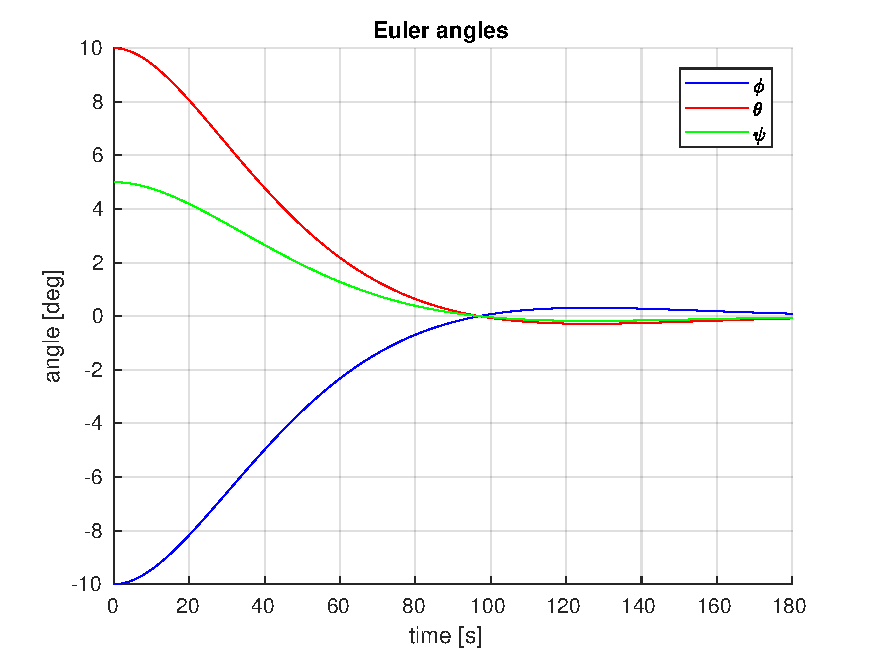
\includegraphics[width=\textwidth]{1_3_euler_angles}
		\caption{Euler angles.}
		\label{fig:2a}
	\end{subfigure}
	~ %add desired spacing between images, e. g. ~, \quad, \qquad, \hfill etc.
	%(or a blank line to force the subfigure onto a new line)
	\begin{subfigure}[b]{0.45\textwidth}
		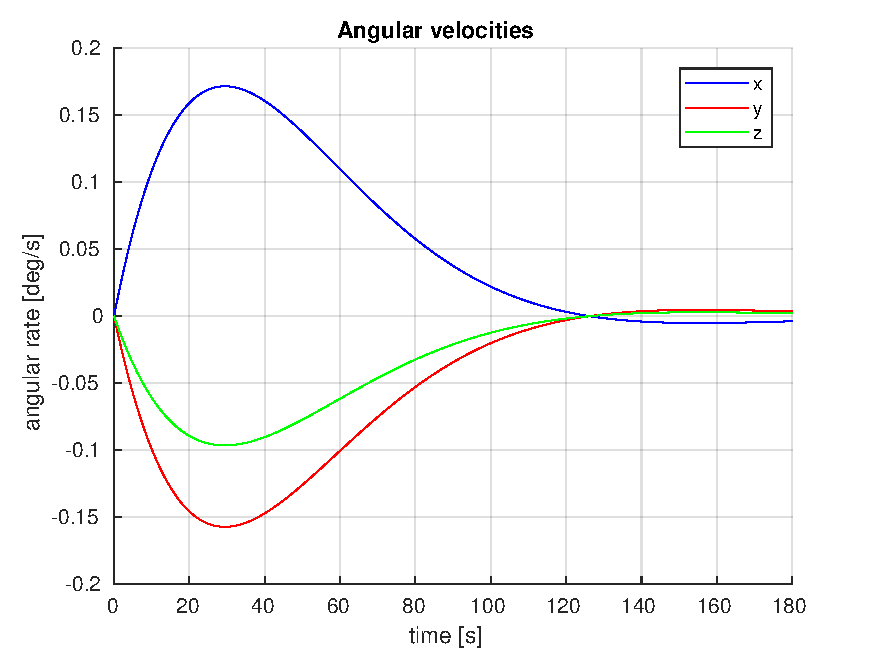
\includegraphics[width=\textwidth]{1_3_angular_velocities}
		\caption{Angular velocities.}
		\label{fig:2b}
	\end{subfigure}
	\begin{subfigure}[b]{0.45\textwidth}
		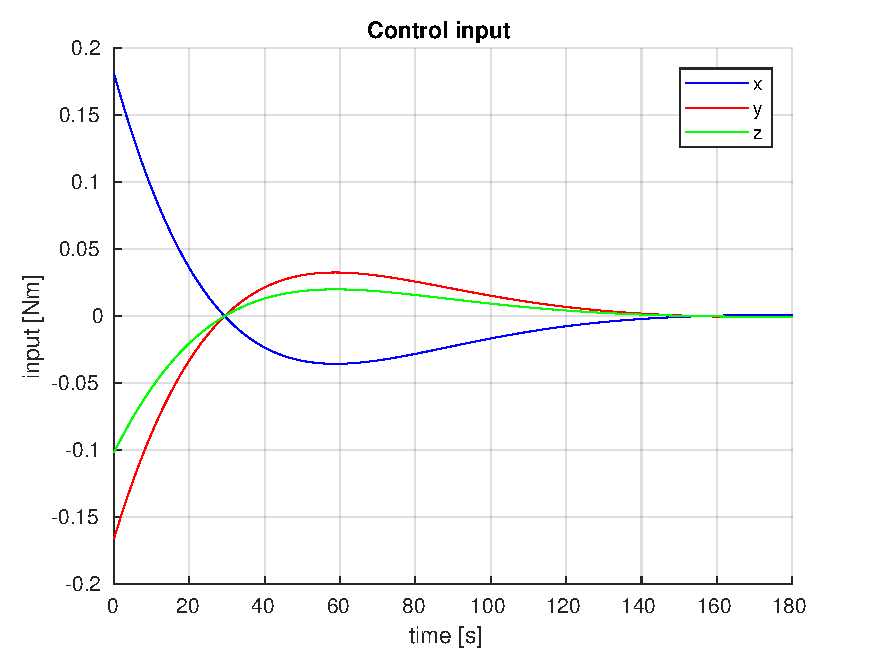
\includegraphics[width=\textwidth]{1_3_control_input}
		\caption{Control input.}
		\label{fig:2c}
	\end{subfigure}
	\caption{Simulation results with control law \eqref{eq:control_law}}\label{fig:zero_control_law}
\end{figure}

\subsection{}
To make a control law based on deviation from a reference, we define the quaternion error
 \begin{equation}
	 \tilde{\mathbf{q}} := \left[
	 \begin{array}{c}
		 \tilde{\eta} \\
		 \tilde{\epsilon}
	 \end{array}
	 \right] = \bar{\mathbf{q}}_d \otimes \mathbf{q},
 \end{equation}
where $\mathbf{q}_d$ is the reference (and the bar denotes the quaternion conjugate). Using the definition of the quaternion product from the assignment text, we obtain
\begin{equation}\begin{aligned}
\tilde{\mathbf{q}} =
\begin{bmatrix}
\eta_d \eta + \boldsymbol{\epsilon}^\top_d \boldsymbol{\epsilon}\\
\eta_d \boldsymbol{\epsilon} - \eta \boldsymbol{\epsilon}_d - \mathbf{S}(\boldsymbol{\epsilon}_d)\boldsymbol{\epsilon}\\
\end{bmatrix}
=
\begin{bmatrix}
\eta_d \eta + \epsilon_{d1} \epsilon_1 + \epsilon_{d2}\epsilon_2 + \epsilon_{d3}\epsilon_3\\
\eta_d \epsilon_1 - \eta \epsilon_{d1} - \epsilon_{d2} \epsilon_3 + \epsilon_{d3}\epsilon_2 \\
\eta_d \epsilon_2 - \eta \epsilon_{d2} - \epsilon_{d3} \epsilon_1 + \epsilon_{d1}\epsilon_3 \\
\eta_d \epsilon_3 - \eta \epsilon_{d3} - \epsilon_{d1} \epsilon_2 + \epsilon_{d2}\epsilon_1 \\
\end{bmatrix}
\end{aligned}\end{equation}
where we have used
\begin{equation}\begin{aligned}
\mathbf{S}(\epsilon_d)\epsilon =
\begin{bmatrix}
0 & -\epsilon_{d3} & \epsilon_{d2}\\
\epsilon_{d3} & 0 & -\epsilon_{d1} \\
-\epsilon_{d2} & \epsilon_{d1} & 0 \\
\end{bmatrix}
\begin{bmatrix}
\epsilon_1\\
\epsilon_2\\
\epsilon_3\\
\end{bmatrix}
=
\begin{bmatrix}
\epsilon_{d2} \epsilon_3 - \epsilon_{d3}\epsilon_2\\
\epsilon_{d3} \epsilon_1 - \epsilon_{d1}\epsilon_3\\
\epsilon_{d1} \epsilon_2 - \epsilon_{d2}\epsilon_1\\
\end{bmatrix}.
\end{aligned}\end{equation}
After convergence, i.e. when $\mathbf{q} = \mathbf{q}_d$, this error becomes
\begin{equation}\begin{aligned}
\tilde{\mathbf{q}} =
\begin{bmatrix}
\eta_d^2 + \boldsymbol{\epsilon}^\top_d \boldsymbol{\epsilon}_d\\
\eta_d \boldsymbol{\epsilon}_d - \eta_d \boldsymbol{\epsilon}_d - \mathbf{S}(\boldsymbol{\epsilon}_d)\boldsymbol{\epsilon}_d\\
\end{bmatrix}
=
\begin{bmatrix}
1\\
\mathbf{0}\\
\end{bmatrix}
\end{aligned}\end{equation}
since $\eta^2 = 1 - \boldsymbol{\epsilon}^\top \boldsymbol{\epsilon}$ and $\boldsymbol{\mathbf{S}}(\boldsymbol{\epsilon})\boldsymbol{\epsilon} = \mathbf{0}$.

\subsection{Problem 1.5}
In problems with simulations, you need to include figures in the report:
\begin{figure}[ht]
	\centering
	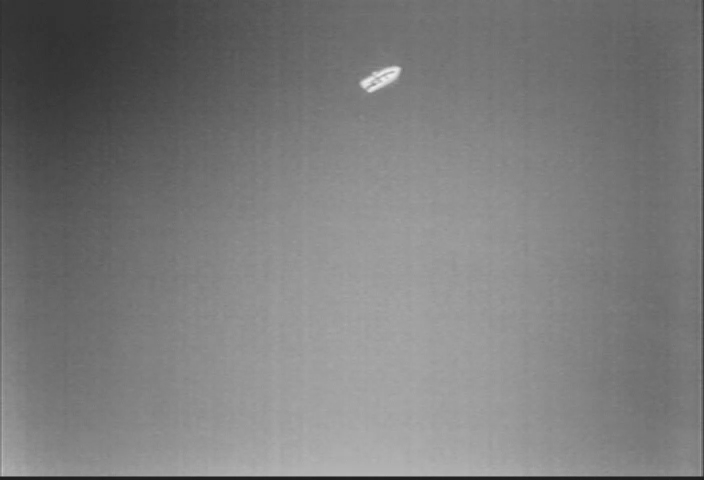
\includegraphics[width=0.7\textwidth]{fig1} % Filename is "fig1.png" and must be located in the same folder as this file. If you have a folder containing all the figures you can use "Figures/fig 1" as long as the "Figures" folder is placed in the same folder as this file.
	\caption{Figure of something useful.}
	\label{fig:fig1}
\end{figure}

You can now refer to this figure as \figref{fig:fig1}. You can also insert figures side-by-side as in Figure \ref{fig:2}. %Notice that \figref includes the word Figure before the reference. If you use "\ref", you need to write the word Figure yourself.
\begin{figure}[ht]
	\centering
	\begin{subfigure}[b]{0.45\textwidth}
		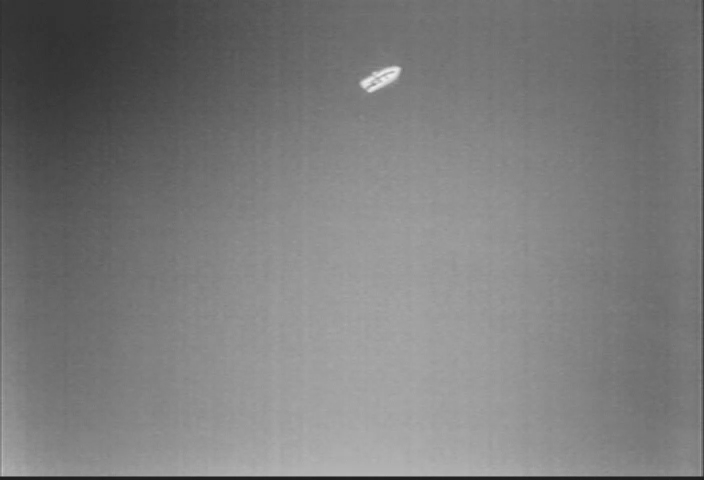
\includegraphics[width=\textwidth]{fig1}
		\caption{caption..}
		\label{fig:2a}
	\end{subfigure}
	~ %add desired spacing between images, e. g. ~, \quad, \qquad, \hfill etc.
	%(or a blank line to force the subfigure onto a new line)
	\begin{subfigure}[b]{0.45\textwidth}
		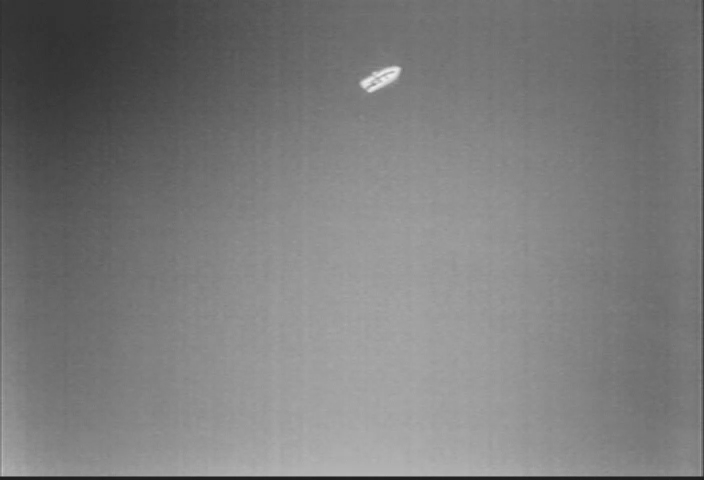
\includegraphics[width=\textwidth]{fig1}
		\caption{caption..}
		\label{fig:2b}
	\end{subfigure}
	\begin{subfigure}[b]{0.45\textwidth}
		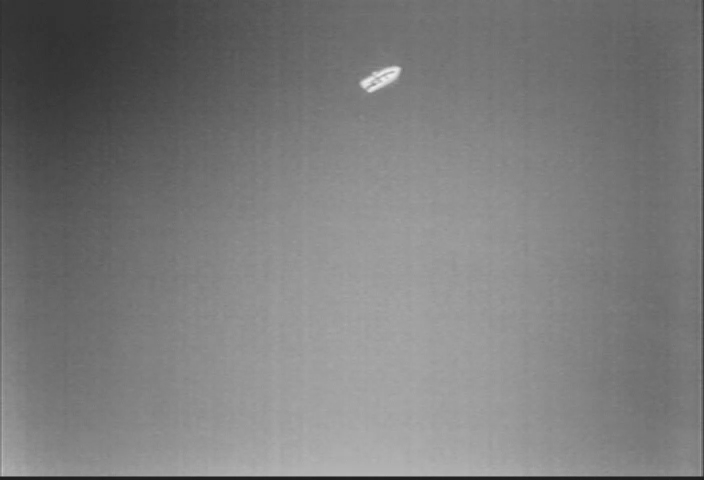
\includegraphics[width=\textwidth]{fig1}
		\caption{caption..}
		\label{fig:2c}
	\end{subfigure}
	\begin{subfigure}[b]{0.45\textwidth}
		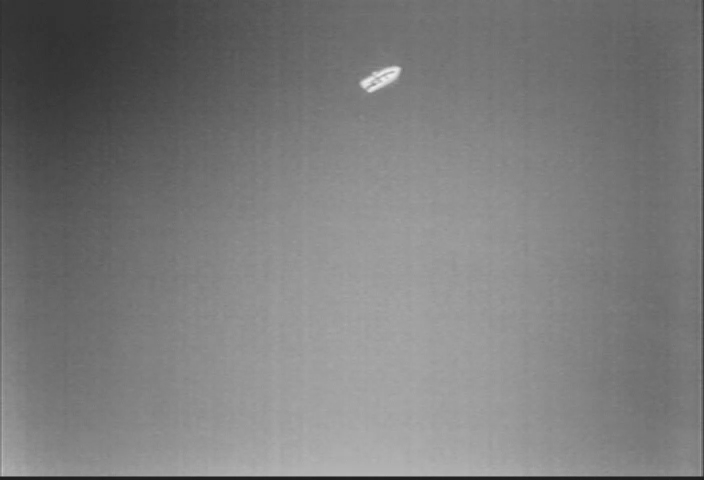
\includegraphics[width=\textwidth]{fig1}
		\caption{caption..}
		\label{fig:2d}
	\end{subfigure}
	\caption{Caption for all figures}\label{fig:2}
\end{figure}


\subsection{Problem 1.6}
The control law in this problem can be written as
\begin{equation}
	\boldsymbol{\tau} = -\mathbf{K}_d \tilde{\boldsymbol{\omega}} - k_p \tilde{\boldsymbol{\epsilon}}
\end{equation}
and the desired angular velocity as
\begin{equation}
	\boldsymbol{\omega}_d = \mathbf{T}^{-1}_{\Theta_d}(\Theta_d)\dot{\Theta}_d
\end{equation}

\subsection{Problem 1.7}
The Lyapunov function can be written as
 \begin{equation}
	 V = \frac{1}{2} \tilde{\boldsymbol{\omega}}^{\top} \mathbf{I}_{CG}\tilde{\boldsymbol{\omega}} + 2 k_p (1-\tilde{\eta})
 \end{equation}
and the derivative as
\begin{equation}
	\dot{V} = -k_d \boldsymbol{\omega}^{\top} \boldsymbol{\omega}
\end{equation}

% Note that \mathbf can be used for bold letters in math mode (within equations and dollar signs). \boldsymbol can be used to get bold greek letters.
